\documentclass[11pt,psfig]{article}
\usepackage{epsfig}
\usepackage{times}
\usepackage{amssymb}
\usepackage{float}

\newcount\refno\refno=1
\def\ref{\the\refno \global\advance\refno by 1}
\def\ux{\underline{x}}
\def\uw{\underline{w}}
\def\bw{\underline{w}}
\def\ut{\underline{\theta}}
\def\umu{\underline{\mu}} 
\def\bmu{\underline{\mu}} 
\def\be{p_e^*}
\newcount\eqnumber\eqnumber=1
\def\eq{\the \eqnumber \global\advance\eqnumber by 1}
\def\eqs{\eq}
\def\eqn{\eqno(\eq)}

 \pagestyle{empty}
\def\baselinestretch{1.1}
\topmargin1in \headsep0.3in
\topmargin0in \oddsidemargin0in \textwidth6.5in \textheight8.5in
\begin{document}
\setlength{\parskip}{1.2ex plus0.3ex minus 0.3ex}


\thispagestyle{empty} \pagestyle{myheadings} \markright{G}



\title{CS 266 Homework 8}
\author{Zachary DeStefano, PhD Student, 15247592}
\date{Due Date: June 5, 2014}

\maketitle

\vfill\eject

\section*{Problem 11.2}

Prove that the worst case running time of algorithm CONVEXHULL is
O(n3), and that there are sets of points where a bad choice of the random
permutation makes the algorithm actually need Θ(n3) time.

%\begin{figure}[H]
%\centering
%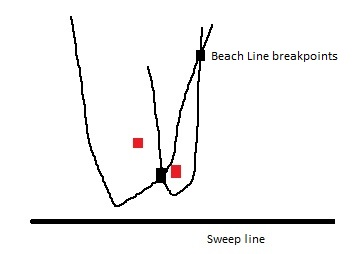
\includegraphics[height=2.5in]{hw7prob1diagram.jpg}
%\caption{Beach Line example. The top breakpoint will move up while the bottom one will move down.}
%\end{figure}

\section*{Problem 11.4}

In many applications, only a small percentage of the points in a given set
P of n points are extreme. In such a case, the convex hull of P has less
than n vertices. This can actually make our algorithm CONVEXHULL
run faster than Θ(nlogn).\\

Assume, for instance, that the expected number of extreme points in a
random sample of P of size r is $O(r^\alpha)$, for some constant $\alpha < 1$. (This
is true when the set P has been created by picking points uniformly at
random in a ball.) Prove that under this condition, the running time of
the algorithm is O(n).

\section*{Problem 11.8}

Describe a randomized incremental algorithm to compute the intersection
of half-planes, and analyze its expected running time. Your algorithm
should maintain the intersection of the current set of half-planes.
To figure out where to insert a new half-plane, maintain a conflict graph
between the vertices of the current intersection and the half-planes that
are still to be inserted.

\end{document}








